\documentclass{article}
\usepackage[utf8]{inputenc}
\usepackage{xcolor}
\usepackage{amsmath}
\usepackage{scrextend}
\usepackage{listings}
\usepackage{tcolorbox}
\usepackage{graphicx}
\usepackage{tikz}
\usepackage{float}
\usepackage{hyperref}
\usepackage[framemethod=tikz]{mdframed}

\setlength{\parindent}{0pt}
\setlength{\parskip}{12pt}
\setlength{\intextsep}{0pt plus 2pt}

% For setting margins
\usepackage[margin=2in]{geometry}


\definecolor{codeColor}{HTML}{282c34}
\definecolor{keyWord}{HTML}{0000ff}
\definecolor{variable}{HTML}{ffffff}
\definecolor{CommentColor}{HTML}{aaaaaa}
\definecolor{StrColor}{HTML}{00ff00}
\definecolor{ruleColor}{HTML}{282c34}

\graphicspath{{.}}

\lstset{backgroundcolor=\color{codeColor}, 
        basicstyle=\fontfamily{pcr}\selectfont\footnotesize\color{variable},
        commentstyle=\color{CommentColor},
        stringstyle=\color{StrColor},
        breaklines=true, 
        rulecolor=\color{codeColor}}

\title{Assignment 4}
\date{}
\author{Jonas Valfridsson\\199608275377}

\begin{document}

\maketitle

As usual All code can be found \href{https://github.com/DD2360-Assignments-Jonas-Valfridsson/Assignments}{https://github.com/DD2360-Assignments-Jonas-Valfridsson/Assignments}
\tableofcontents

\newpage  

\section{Hello World}%
\label{sec:hello_world}



My first Kernel looked like this

\begin{mdframed}[backgroundcolor=codeColor,leftmargin=0.0cm,hidealllines=true,%
  innerleftmargin=0.1cm,innerrightmargin=0.1cm,innertopmargin=0.5cm,innerbottommargin=0.10cm,
  roundcorner=15pt]
\begin{lstlisting}[language=C]
  __kernel void hello_world () {                                                                                                                                             
      int index = get_global_id(0);                                                                                                     
      printf("Hello World! My threadId is %d\n", index);                                                                                                                                                                                 
  }                                                      
\end{lstlisting}
\end{mdframed}

This gave the expected output printing thread ID from 0 $\rightarrow 255$

Now for the first modification I modified my program to have a 16x16 distribution, I had to update my kernel launch code to

\begin{mdframed}[backgroundcolor=codeColor,leftmargin=0.0cm,hidealllines=true,%
  innerleftmargin=0.1cm,innerrightmargin=0.1cm,innertopmargin=0.5cm,innerbottommargin=0.10cm,
  roundcorner=15pt]
\begin{lstlisting}[language=C]
    const size_t kernel_dim = 2;
    size_t n_workitem[kernel_dim];
  
    n_workitem[0] = 16;
    n_workitem[1] = 16;
  
    size_t workgroup_size[kernel_dim];
    workgroup_size[0] = 1;
    workgroup_size[1] = 1;
  
    err = clEnqueueNDRangeKernel(cmd_queue, kernel, 
        kernel_dim, NULL, n_workitem, workgroup_size, 0, NULL, NULL);CHK_ERROR(err);
\end{lstlisting}
\end{mdframed}

And I updated my kernel to

\begin{mdframed}[backgroundcolor=codeColor,leftmargin=0.0cm,hidealllines=true,%
  innerleftmargin=0.1cm,innerrightmargin=0.1cm,innertopmargin=0.5cm,innerbottommargin=0.10cm,
  roundcorner=15pt]
\begin{lstlisting}[language=C]
  __kernel void hello_world () {
      int x = get_global_id(0);
      int y = get_global_id(1);
      printf("Hello World! My threadId is (%d, %d)\n", x, y);
  }
\end{lstlisting}
\end{mdframed}

\newpage 
For the second modification I now modified my code to run the 16x16 grid in 4x4 work-groups. For this I first modified my kernel launch to

\begin{mdframed}[backgroundcolor=codeColor,leftmargin=0.0cm,hidealllines=true,%
  innerleftmargin=0.1cm,innerrightmargin=0.1cm,innertopmargin=0.5cm,innerbottommargin=0.10cm,
  roundcorner=15pt]
\begin{lstlisting}[language=C]
    const size_t kernel_dim = 2;
    size_t n_workitem[kernel_dim];
  
    n_workitem[0] = 16;
    n_workitem[1] = 16;
  
    size_t workgroup_size[kernel_dim];
    workgroup_size[0] = 4;
    workgroup_size[1] = 4;
  
    err = clEnqueueNDRangeKernel(cmd_queue, kernel, 
        kernel_dim, NULL, n_workitem, workgroup_size, 0, NULL, NULL);CHK_ERROR(err);
\end{lstlisting}
\end{mdframed}

And I updated my kernel to

\begin{mdframed}[backgroundcolor=codeColor,leftmargin=0.0cm,hidealllines=true,%
  innerleftmargin=0.1cm,innerrightmargin=0.1cm,innertopmargin=0.5cm,innerbottommargin=0.10cm,
  roundcorner=15pt]
\begin{lstlisting}[language=C]
 __kernel void hello_world () {                                                             
     int local_x = get_local_id(0);                            
     int local_y = get_local_id(1);                            
                                                               
     int group_x = get_group_id(0);                            
     int group_y= get_group_id(1);                             
                                                               
     int x_size = get_local_size(0);                           
     int y_size = get_local_size(1);                           
                                                               
     int x = local_x + x_size * group_x;                       
     int y = local_y + y_size * group_y;                       
                                                               
     printf("Hello World! My threadId is (%d, %d)\\n", x, y);
 }                                                             

\end{lstlisting}
\end{mdframed}

\newpage
For the third modifications I now modified my code to run a 3x3x3 grid in a 1x1x1 work-group. For this I modified my kernel launch to

\begin{mdframed}[backgroundcolor=codeColor,leftmargin=0.0cm,hidealllines=true,%
  innerleftmargin=0.1cm,innerrightmargin=0.1cm,innertopmargin=0.5cm,innerbottommargin=0.10cm,
  roundcorner=15pt]
\begin{lstlisting}[language=C]
    const size_t kernel_dim = 3;
    size_t n_workitem[kernel_dim];
  
    n_workitem[0] = 3;
    n_workitem[1] = 3;
    n_workitem[2] = 3;
  
    size_t workgroup_size[kernel_dim];
    workgroup_size[0] = 1;
    workgroup_size[1] = 1;
    workgroup_size[2] = 1;
  
    err = clEnqueueNDRangeKernel(cmd_queue, kernel, 
        kernel_dim, NULL, n_workitem, workgroup_size, 0, NULL, NULL);CHK_ERROR(err);
\end{lstlisting}
\end{mdframed}

Then I modified my kernel to

\begin{mdframed}[backgroundcolor=codeColor,leftmargin=0.0cm,hidealllines=true,%
  innerleftmargin=0.1cm,innerrightmargin=0.1cm,innertopmargin=0.5cm,innerbottommargin=0.10cm,
  roundcorner=15pt]
\begin{lstlisting}[language=C]
  __kernel void hello_world () {                                                                     
      int x = get_global_id(0);                                         
      int y = get_global_id(1);                                         
      int z = get_global_id(2);                                         
                                                                        
      printf("Hello World! My threadId is (%d, %d, %d)\n", 
             x, y, z); 
  }                                                                     
\end{lstlisting}
\end{mdframed}

\newpage 
\section{SAXPY}%
\label{sec:hello_world}

I solved ARRAY\_SIZE not being a multiple of block size in the same way I did in Cuda. I added one additional block to the execution and a bounds check to my kernel. My kernel looked like so:

\begin{mdframed}[backgroundcolor=codeColor,leftmargin=0.0cm,hidealllines=true,%
  innerleftmargin=0.1cm,innerrightmargin=0.1cm,innertopmargin=0.5cm,innerbottommargin=0.10cm,
  roundcorner=15pt]
\begin{lstlisting}[language=C]
  __kernel void saxpy (  __global long *n,            
                         __global float *x,           
                         __global float *a,           
                         __global float *y) {                                            
      int index = get_global_id(0);            
      if (index < *n)                          
        y[index] = (*a) * x[index] + y[index]; 
  }                                            
\end{lstlisting}
\end{mdframed}

I also did benchmark

\begin{figure}[H]
  \centering
  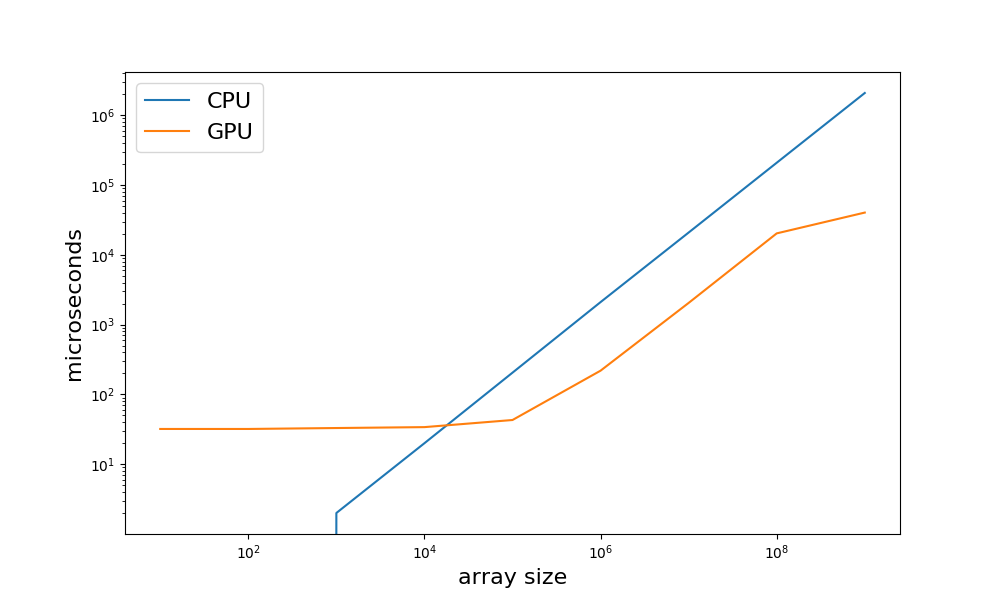
\includegraphics[width=0.95\linewidth]{ex_2/saxpy-cpu-vs-gpu.png}
  \caption{SAXPY OpenCL}
  \label{fig:}
\end{figure}

Comparing it to my CUDA benchmark

\begin{figure}[H]
  \centering
  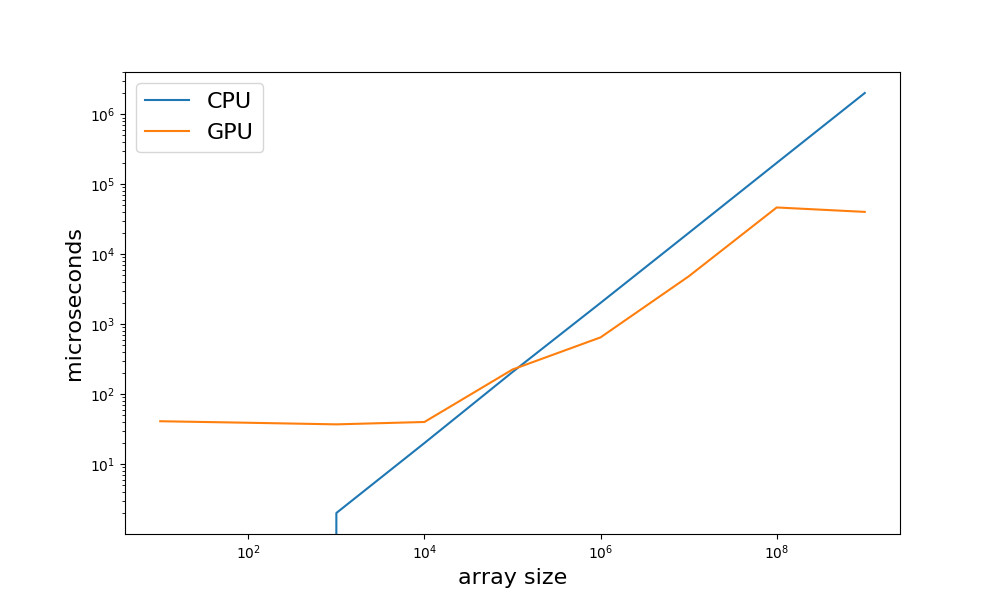
\includegraphics[width=0.95\linewidth]{ex_2/saxpy-cpu-vs-gpu-cuda.png}
  \caption{SAXPY Cuda}
  \label{fig:}
\end{figure}

They are very similar, expect that the CUDA seems to be doing a bit better with the largest arrays. But this might just be because the way I am benchmarking is maybe not optimal.

\section{Discuss Reflect Contrast}%
\label{sec:discuss_reflect_contrast}

I really don't like that OpenCL does runtime compilation, I think that is a horrible pattern. The fact that OpenCL promises to work across so many devices is what makes it attractive though. But I am wondering if writing for
OpenCL once or just writing once per usable device would be the approach I take, since you still have to do so many device checks in OpenCL. 

For me personally I would not use OpenCL in its current state, the run-time compilation really turned me off. I much prefer Cuda in that aspect - and if I ever use other GPUs or devices i'll just have to port my code, which
I believe will be fine. Performance-wise OpenCL and Cuda was very similar for me, potentially Cuda was a little faster but that might have just been variance in my benchmarks.

\end{document}




